\chead{\textit{Application}}  				
\section{Application}

%TODO Write introduction to chapter

\subsection{Modeling Framework}
\label{sec:app:mod-framework}

This section introduces the reader to all relevant information about the modelling framework that is used to model a real-life application. The modelling framework has to cover certain requirements. Firstly, there should be generators that produce electrical power. The power output is only limited by the maximum capacity of the generator. There exist no ramping constraints or minimum up- and down-times. Each generator has marginal costs and is connected to a specific node. To depict these requirements in Julia, a generator structure was implemented as you can see in the following code snippet. In addition to the stated requirements, the structure also contains a colour and a name. These attributes are mainly used for evaluation reasons and are not important for modelling purposes. 

\lstinputlisting[language=julia, firstline=7, lastline=13, caption=Julia structure for a node element]{../src/structures/network_elements.jl}

Another part of the modelling framework is a storage unit. Storages should be able to store a surplus of energy as well as deliver electrical power by discharging their capacity. The power input and output is also limited. In addition, a storage unit should only be able to store a certain amount of energy. This is depicted by the storage level. As generators, storages have specific marginal costs for charging and discharging and are connected to a specific node. A Julia structure was implemented respectively.\\

As written before, generators and storages are located at network nodes. These nodes have a specific demand that should be matched by the output of the generating units. For modelling purposes, it is also crucial to define a slack node to compensate the power flow balance. The node structure was implemented as follows:

\lstinputlisting[language=julia, firstline=1, lastline=5, caption=Julia structure for a generator element]{../src/structures/network_elements.jl}

The last element of the framework is a transmission line. This element connects nodes and enables the exchange of energy. Transmission lines are characterized by their maximum capacity and their susceptance value. However, susceptance might not be the correct term here since the model does not consider alternating current. Thus, the correct name would be conductance but is not used to follow general naming conventions. A Julia structure was also implemented for this network element.\\

Lastly, the modelling framework has to consider multi-periods. This is crucial since without multi periods, it would not make sense to include storages into the system.\\

All structures are defined in \path{src\structures\network_elements.jl} and can be found in \ref{app:jl:ne}.

 
\subsection{Three Node System}
\label{sec:app:tns}
% Move after mathematical formulations and implementation and then write equations again for this example

The following section describes the \gls{tns} which will be used throughout the chapter to derive the optimization the model. The system consists of three nodes. At each of them, a different set of generators and storages is located. Each node has a different multi-period demand vector. To simplify the equations and make them easier to understand, only two time steps are considered. The nodes are connected by a total of three transmission lines. Thus, every node has two neighbours. All network elements must meet the requirements described in section (\ref{sec:app:mod-framework}). The network layout is shown in figure (\ref{fig:tns}).

%TODO Make own graphic for three node system
\begin{figure}[h]
	\centering
	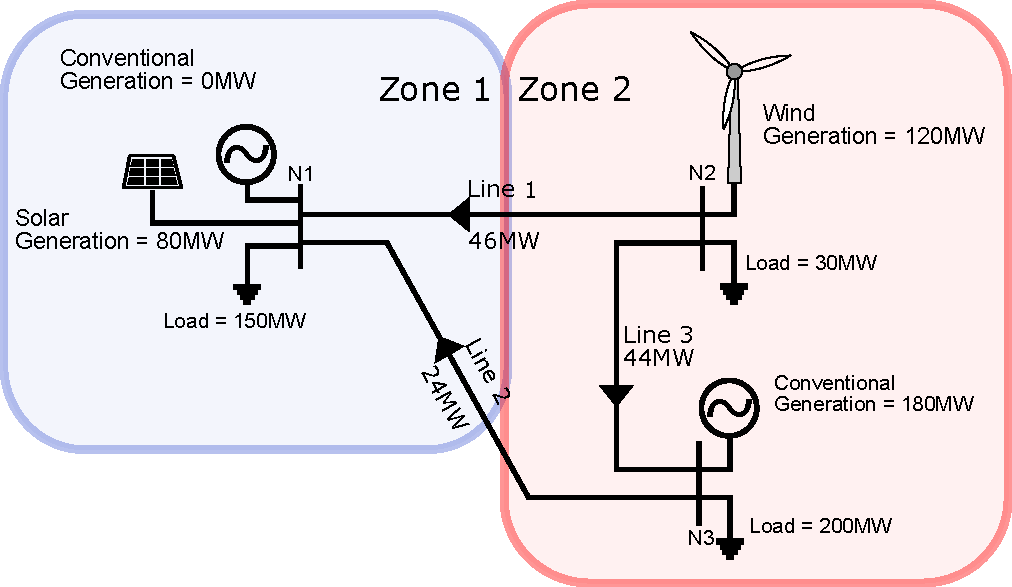
\includegraphics[width=0.8\textwidth]{three-node-system.png}
	\caption{Exemplary Three Node System}
	\label{fig:tns}
\end{figure}


\subsection{Mathematical formulations}

As written in the introduction, the aim of this thesis is to develop a framework to minimize the total system costs of a electrical network in a decentralized manner. This means that the costs are optimized without a central entity. Thus, the generating units are able to derive their own optimal decisions without releasing sensible information like their marginal costs. This section presents the mathematical formulations of the optimization problem. Since the solution of the decentralized problem will be compared with the solution of the centralized problem and the decentralized problem is based on the centralized problem, the centralized optimization model is introduced first.

\subsubsection{Centralized optimization problem}

The total system costs of a electrical network like the one in section \ref{sec:app:tns} are the sum of generation costs of all participating units over all time steps. With regard to the modeling framework, this means that the system costs are composed of the generator costs and the storage costs. The centralized optimization problem can be formulated as follows:

\begin{subequations}
	\begin{align}
		 \min \quad & \sum_{t\in\mathcal{T}}\sum_{g\in\mathcal{G}}c_g*P_g(t) + \sum_{s\in\mathcal{S}}c_s*(P_s^d(t)+P_s^c(t))\\
		 \text{s.t. } \quad & 0 \leq P_g(t) \leq \overline{P_g} && \forall g \in \set{G}, t \in \set{T} \label{eq:com:con:max-g}\\
		 & 0 \leq P_s^d(t) \leq \overline{P_s} && \forall s \in \set{S}, t \in \set{T} \label{eq:com:con:max-sd}\\
		 & 0 \leq P_s^c(t) \leq \overline{P_s} && \forall s \in \set{S}, t \in \set{T} \label{eq:com:con:max-sc}\\
		 & 0 \leq E_s(t) \leq \overline{E_s} && \forall s \in \set{S}, t \in \set{T} \label{eq:com:con:s-level-max}\\
		 & E_s(t) - E_s(t-1) - P_s^c(t) + P_s^d(t) = 0 && \forall s \in \set{S}, t \in \set{T} \label{eq:com:con:s-level}\\
		 & I_n(t) = \sum_{g\in\mathcal{G}}P_g(t) + \sum_{s\in\mathcal{S}}(P_s^d(t)-P_s^c(t))-D_n(t) = 0 && \forall t \in \set{T}, n \in \set{N} \label{eq:com:con:eb}\\
		 & -\overline{L_l} \leq PTDF * I_n(t) \leq \overline{L_l} && \forall l \in \set{L}, t \in \set{T}, n \in \set{N} \label{eq:com:con:pf}
	\end{align}
\end{subequations}

Hereby, $\mathcal{G}$ represents the set of generators and $\mathcal{S}$ the set of storage respectively. $\mathcal{T}$ includes all considered timesteps. The optimization problem is constrained to meet the requirements written in section (\ref{sec:app:mod-framework}). First of all, equation (\ref{eq:com:con:max-g}) limits the maximum output of all generators where $\overline{P_g}$ is the maximum power generation of the considered generator. Equations (\ref{eq:com:con:max-sd}) and (\ref{eq:com:con:max-sc}) set the boundaries of all storages and equation (\ref{eq:com:con:s-level-max}) ensures that the storage level of all storages remains between zero and the maximum storage level $\overline{E_s}$. The storage level at a specific time step can be calculated as follows:

\begin{equation}
	\label{eq:storage-level}
	E_s(t) = E_s(t-1) + P_s^c(t) - P_s^d(t)
\end{equation}

To get a consistent form of all constraints, equation (\ref{eq:storage-level}) is rearranged to equal zero and integrated in the optimization problem as equation (\ref{eq:com:con:s-level}). Hereby, $P_s^c(t)$ denotes the charging output of a storage $s$ at a timestep $t$ and $P_s^d(t)$ the discharging output. Equation (\ref{eq:com:con:eb}) is the so called energy balance. This constraint ensures that the demand at every node and every time step is met. The energy balance is also referred to as the injection at node $n$ at time step $t$. The injection term is used in the last constraint (\ref{eq:com:con:pf}) that establishs the network constraints. Here, the power flows on each transmission line are limited by the maximum line capacity $\overline{L_l}$. The line utilization for each transmission line is calculated by multiplying the \gls{ptdf} with the injection term $I_n(t)$.\\

	%TODO Explain PTDF, see maybe document from EMOD.
	
To solve the optimization problem, all relevant information has to be shared with the central entity. In the example above this includes marginal costs and the maximal capacities of the generating units. The central entity is then able to derive the optimal dispatch plan that minimizes the total system costs and informs the generating units about their generation schedule. Thus, the generating units are not able to optimize their decision on their own because the central entity is needed for coordination.	

\subsubsection{Decentralized optimization problem}

% TODO Add reference for ADMM explanation
The generating units in the centralized optimization problem are not able to optimize on their own because a central entity is needed to coordinate the system constraints (\ref{eq:com:con:eb}) and (\ref{eq:com:con:pf}). These constraints prevent that the solution is obtained by optimizing per generating unit because both include all decision variables of the optimization problem. This is the reason why these constraints are called complicating constraints. If resolved, it would be possible to derive the optimal dispatch plan per generating unit and without sharing sensible information like marginal costs. As written in \ref{admm}, the \gls{admm} provides a technique to resolve these constraints, making the problem decomposable and thus enables the path to a decentralized mechanism. \gls{admm} is only working for equality constraints. Thus, the power flow inequality constraint (\ref{eq:com:con:pf}) is transformed into two equality constraints by introducing two slack variables $R^{ref}_l$ and $R^{cref}_l$ for each tranmission line $l$. The optimization problem evolves to the following:

\begin{subequations}
	\begin{align}
		 \min \quad & \sum_{t\in\mathcal{T}}\sum_{g\in\mathcal{G}}c_g*P_g(t) + \sum_{s\in\mathcal{S}}c_s*(P_s^d(t)+P_s^c(t)) \label{eq:dom:relaxed-constraints}\\
		 \text{s.t.} \quad & 0 \leq P_g(t) \leq \overline{P_g} && \forall g \in \set{G}, t \in \set{T} \\
		 & 0 \leq P_s^d(t) \leq \overline{P_s} && \forall s \in \set{S}, t \in \set{T} \\
		 & 0 \leq P_s^c(t) \leq \overline{P_s} && \forall s \in \set{S}, t \in \set{T} \\
		 & 0 \leq E_s(t) \leq \overline{E_s} && \forall s \in \set{S}, t \in \set{T} \\
		 & E_s(t) - E_s(t-1) - P_s^c(t) + P_s^d(t) = 0 && \forall s \in \set{S}, t \in \set{T} \\
		 & I_n(t) = \sum_{g\in\mathcal{G}}P_g(t) + \sum_{s\in\mathcal{S}}(P_s^d(t)-P_s^c(t))-D_n(t) = 0 && \forall t \in \set{T}, n \in \set{N} \\
		 & PTDF * I_n(t) + R^{ref}_l - \overline{L_l} = 0 && \forall l \in \set{L}, t \in \set{T}, n \in \set{N} \label{eq:dom:con:pf-upper} \\
		 & R^{cref}_l - PTDF * I_n(t) - \overline{L_l} = 0 && \forall l \in \set{L}, t \in \set{T}, n \in \set{N} \label{eq:dom:con:pf-lower}
	\end{align}
\end{subequations}

The slack variable $R_l^{ref}$ ensures that the upper bound of the transmission line capactiy is kept, while slack variable $R_l^{cref}$ ensures the lower limit. Both variables are added as additional decision variables. Instead of two complicating constraints, one has to handle three complicating constraints. If these constraints are relaxed, the main problem decomposes into a generator and a storage subproblem.\\

Relaxing the complicating variables is done by implementing a max-min problem using the dual variables of the complicated constraints. Hereby, $\lambda$ is the dual of the energy balance constraint, $\mu$ and $\rho$ are the duals of the upper and lower power flow constraint respectively. Since the objective function is a linear cost function, \gls{lr} is not applicable. Thus, the complicated constraints are relaxed by applying \gls{alr}. A penalty term for each dual variable is introduced. The penalty terms equal zero in the optimality point and contribute to a faster convergence. The optimization problem of (\ref{eq:dom:relaxed-constraints}) derives to:

\begin{subequations}
	\begin{align}
		\max{(\lambda, \mu, \rho)} \label{eq:dom:fixed-duals} \\
		 & \min \quad \sum_{t\in\mathcal{T}}\sum_{g\in\mathcal{G}}c_g*P_g(t) + \sum_{s\in\mathcal{S}}c_s*(P_s^d(t)+P_s^c(t)) \nonumber \\
		 & + \lambda * \left[\sum_{g\in\mathcal{G}}P_g(t) + \sum_{s\in\mathcal{S}}(P_s^d(t)-P_s^c(t))-D_n(t)\right]\nonumber \\
		 & + \frac{\gamma}{2} * \left[\sum_{g\in\mathcal{G}}P_g(t) + \sum_{s\in\mathcal{S}}(P_s^d(t)-P_s^c(t))-D_n(t)\right]^2 \nonumber \\
		 & + \mu * \left[PTDF * I_n(t) + R^{ref}_l - \overline{L_l}\right] \nonumber \\
		 & + \frac{\gamma}{2} * \left[PTDF * I_n(t) + R^{ref}_l - \overline{L_l}\right]^2 \nonumber \\
		 & + \rho * \left[R^{cref}_l - PTDF * I_n(t) - \overline{L_l}\right]\nonumber
	\end{align}
	\begin{align}
		 \text{s.t. } \quad & 0 \leq P_g(t) \leq \overline{P_g} && \forall g \in \set{G}, t \in \set{T}\\\
		 & 0 \leq P_s^d(t) \leq \overline{P_s} && \forall s \in \set{S}, t \in \set{T}\\
		 & 0 \leq P_s^c(t) \leq \overline{P_s} && \forall s \in \set{S}, t \in \set{T}\\
		 & 0 \leq E_s(t) \leq \overline{E_s} && \forall s \in \set{S}, t \in \set{T}\\
		 & E_s(t) - E_s(t-1) - P_s^c(t) + P_s^d(t) = 0 && \forall s \in \set{S}, t \in \set{T}
	\end{align}
\end{subequations}

Variable $\gamma$ is a positive constant and is the only parameter needed for the \gls{admm}. Due to the quadratic terms of the relaxed complicating constraitns, the first derivatives of the objective function is not fixed anymore but continuous. This is also a necessary condition for the convergence of the algorithm. Still, the optimization problem in equation (\ref{eq:dom:fixed-duals}) is not decomposable because of the introduced dual variables. The problem is further relaxed by fixing the dual variable to given values $\overline{\lambda}$, $\overline{\mu}$, $\overline{\rho}$. The problem formulation becomes:

\begin{subequations}
	\begin{align}
		 \min \quad & \sum_{t\in\mathcal{T}}\sum_{g\in\mathcal{G}}c_g*P_g(t) + \sum_{s\in\mathcal{S}}c_s*(P_s^d(t)+P_s^c(t)) \label{eq:dom:final} \\
		 & + \overline{\lambda} * \left[\sum_{g\in\mathcal{G}}P_g(t) + \sum_{s\in\mathcal{S}}(P_s^d(t)-P_s^c(t))-D_n(t)\right]\nonumber \\
		 & + \frac{\gamma}{2} * \left[\sum_{g\in\mathcal{G}}P_g(t) + \sum_{s\in\mathcal{S}}(P_s^d(t)-P_s^c(t))-D_n(t)\right]^2 \nonumber \\
		 & + \overline{\mu} * \left[PTDF * I_n(t) + R^{ref}_l - \overline{L_l}\right] \nonumber \\
		 & + \frac{\gamma}{2} * \left[PTDF * I_n(t) + R^{ref}_l - \overline{L_l}\right]^2 \nonumber \\
		 & + \overline{\rho} * \left[R^{cref}_l - PTDF * I_n(t) - \overline{L_l}\right]\nonumber \\
		 & + \frac{\gamma}{2} * \left[R^{cref}_l - PTDF * I_n(t) - \overline{L_l}\right]^2\nonumber \\
		 \text{s.t.} \quad & 0 \leq P_g(t) \leq \overline{P_g} && \forall g \in \set{G}, t \in \set{T}\\\
		 & 0 \leq P_s^d(t) \leq \overline{P_s} && \forall s \in \set{S}, t \in \set{T}\\
		 & 0 \leq P_s^c(t) \leq \overline{P_s} && \forall s \in \set{S}, t \in \set{T}\\
		 & 0 \leq E_s(t) \leq \overline{E_s} && \forall s \in \set{S}, t \in \set{T}\\
		 & E_s(t) - E_s(t-1) - P_s^c(t) + P_s^d(t) = 0 && \forall s \in \set{S}, t \in \set{T}
	\end{align}
\end{subequations}

% TODO Add reference for ADMM explanation
Because of the product of the decision variable $P_{\mathcal{G}}$, $P_{\mathcal{S}}^d$ and $P_{\mathcal{S}}^c$ in all penalty terms, the optimization model is still not decomposable. At this step, the \gls{admm} comes into action and provides a possibility to solve the problem in a decomposable way. As written in \ref{admm}, \gls{admm} fixes each decision variable to the previous iteration value. Thus, one is finally able to derive the generator and storage subproblem. Out of simplicity, the overline symbol on the dual variables is omitted in the next equations.


\subsubsection*{Generator subproblem}

In the following, the optimization model for a specific generator $g$ is derived. The problem is only optimized by the decision variable $P_{g}$ of a specific generator and the corresponding slack variables. With the help of \gls{admm}, decision variables $P_{\mathcal{S}}^d$ and $P_{\mathcal{S}}^c$ are fixed to the values of the previous iteration. The power output of all other generators $P_{g \notin \mathcal{G}}$ is fixed too. Any constraint related to these variables can be removed. Another parameter $v$ is added to the problem formulation that indicates the iteration number. Obviously, for decision variable $P_{g}$ one takes the current iteration number $v$ while for the storages and other generators one takes the previous iteration $v-1$. The first derivative of the objective function shows that the objective function can be further simplified by removing terms related to $P_{g \notin \mathcal{G}}$, $P_{\mathcal{S}}^d$ and $P_{\mathcal{S}}^c$. The power in the penalty terms prohibits them to be further simplified.

% When writing multi-line equations with the align, align* or aligned environments, the \left and \right commands must be balanced on each line and on the same side of &. The solution is to use "invisible" brackets to balance things out, i.e. adding a \right. at the end of the first line, and a \left. at the start of the second line after &:
\begin{subequations}
	\begin{align}
		 \min \quad & \sum_{t\in\mathcal{T}} c_g*P_g(v, t) + \lambda * P_g(v, t) \\
		 & + \frac{\gamma}{2} * \left[ P_g(v, t) \sum_{g\notin\mathcal{G}}P_g(v-1,t) \right. \nonumber \\
		 & \qquad \left. + \sum_{s\in\mathcal{S}}(P_s^d(v-1, t)-P_s^c(v-1, t))-D_n(t)\right]^2 \\
		 & + \mu * \left[PTDF * P_g(v, t)\right] \nonumber \\
		 & + \frac{\gamma}{2} * \left[PTDF * I_n(v, t) + R^{ref}_l(v) - \overline{L_l}\right]^2 \nonumber \\
		 & + \rho * \left[- PTDF * P_g(v, t)\right] \nonumber \\
		 & + \frac{\gamma}{2} * \left[R^{cref}_l(v) - PTDF * I_n(v, t) - \overline{L_l}\right]^2\nonumber \\
		 \text{s.t.} \quad & 0 \leq P_g(v, t) \leq \overline{P_g} && \forall t \in \set{T}
	\end{align}
\end{subequations}

 

\subsubsection{Matrix Form}

Typically, \gls{admm} solves problems in the form:

\begin{subequations}
	\begin{align}
		\min{(x, z)} \quad & f(x) + g(z) \\
		\text{s.t. } \quad & \vb{A}x + \vb{B}z = c
	\end{align}
\end{subequations}

If applied to the formulation in the section \ref{sec:general_formulation}, the generator problem looks like:

\begin{subequations}
	\begin{align}
		f(x) &= f(\vb{P_\mathcal{G}}) = \vb{P_\mathcal{G}}^T * \va{c_\mathcal{G}}\\
		& = \begin{bmatrix}
			P_{g_1}(t_1) & P_{g_2}(t_1) & P_{g_3}(t_1) \\
			P_{g_1}(t_2) & P_{g_2}(t_2) & P_{g_3}(t_2)
		\end{bmatrix} * \begin{bmatrix}
			c_{g_1} \\
			c_{g_2} \\
			c_{g_3}
		\end{bmatrix} \\
		& = \begin{bmatrix}
			P_{g_1}(t_1) * c_{g_1} + P_{g_2}(t_1) * c_{g_2} + P_{g_3}(t_1) * c_{g_3} \\
			P_{g_1}(t_2) * c_{g_1} + P_{g_2}(t_2) * c_{g_2} + P_{g_3}(t_2) * c_{g_3} \\
		\end{bmatrix}
	\end{align}
\end{subequations}

In addition, the storage problem yields:

\begin{subequations}
	\begin{align}
		g(z) &= g(\vb{P_\mathcal{S}^d}, \vb{P_\mathcal{S}^c})\\
		& = \left(\vb{P_\mathcal{S}^d}^T + \vb{P_\mathcal{S}^c}^T\right) * \va{c_\mathcal{S}} \\
		& = \left(\begin{bmatrix}
			P_{s_1}^d(t_1) & P_{s_2}^d(t_1) \\
			P_{s_1}^d(t_2) & P_{s_2}^d(t_2)
		\end{bmatrix} + \begin{bmatrix}
			P_{s_1}^c(t_1) & P_{s_2}^c(t_1) \\
			P_{s_1}^c(t_2) & P_{s_2}^c(t_2)
		\end{bmatrix} \right) * \begin{bmatrix}
			c_{s_1} \\
			c_{s_2}
		\end{bmatrix} \\
		& = \begin{bmatrix}
			P_{s_1}^d(t_1) + P_{s_1}^c(t_1) & P_{s_2}^d(t_1) + P_{s_2}^c(t_1) \\
			P_{s_1}^d(t_2) + P_{s_1}^c(t_2) & P_{s_2}^d(t_2) + P_{s_2}^c(t_2)
		\end{bmatrix} * \begin{bmatrix}
			c_{s_1} \\
			c_{s_2}
		\end{bmatrix} \\
		& = \begin{bmatrix}
			P_{s_1}(t_1) * c_{s_1} + P_{s_2}(t_1) * c_{s_2} \\
			P_{s_1}(t_2) * c_{s_1} + P_{s_2}(t_2) * c_{s_2} \\
		\end{bmatrix}
	\end{align}
\end{subequations}

Only the energy balance constraint and the constraints for the power flow are part of the \gls{admm} formulation. All the other constraints are either part of the generator problem or of the storage problem and can be easily decomposed. \\

For this example, only generator 2 and storage 2 are located at node 2. The other resources are located at node 1. Then, the energy balance constraint in matrix form yields:

\begin{subequations}
	\begin{align}
		& \vb{N_\mathcal{G}}*\vb{P_\mathcal{G}} + \vb{N_\mathcal{S}}*(\vb{P_\mathcal{S}^d} - \vb{P_\mathcal{S}^c}) - \vb{D_\mathcal{N}} = \vb{I_\mathcal{N}} = \vb{0} \\
		& \Leftrightarrow \begin{bmatrix}
			1 & 0 & 1 \\
			0 & 1 & 0 \\
		\end{bmatrix} * \begin{bmatrix}
				P_{g_1}(t_1) & P_{g_1}(t_2) \\
				P_{g_2}(t_1) & P_{g_2}(t_2) \\
				P_{g_3}(t_1) & P_{g_3}(t_2)
		\end{bmatrix} \\
		& \qquad + \begin{bmatrix}
			1 & 0 \\
			0 & 1 \\
		\end{bmatrix} * \left(\begin{bmatrix}
			P_{s_1}^d(t_1) & P_{s_1}^d(t_2) \\
			P_{s_2}^d(t_1) & P_{s_2}^d(t_2)
		\end{bmatrix} - \begin{bmatrix}
			P_{s_1}^c(t_1) & P_{s_1}^c(t_2) \\
			P_{s_2}^c(t_1) & P_{s_2}^c(t_2)
		\end{bmatrix} \right) \nonumber \\
		& \qquad - \begin{bmatrix}
			D_{n_1}(t_1) & D_{n_1}(t_2) \\
			D_{n_2}(t_1) & D_{n_2}(t_2)
		\end{bmatrix} = \begin{bmatrix}
			0 & 0 \\
			0 & 0
		\end{bmatrix} \nonumber \\
		& \Leftrightarrow \begin{bmatrix}
				P_{g_1}(t_1) + P_{g_3}(t_1) & P_{g_1}(t_2) + P_{g_3}(t_2) \\
				P_{g_2}(t_1) & P_{g_2}(t_2)
		\end{bmatrix} + \begin{bmatrix}
			P_{s_1}^d(t_1) - P_{s_1}^c(t_1) & P_{s_1}^d(t_2) - P_{s_1}^c(t_2) \\
			P_{s_2}^d(t_1) - P_{s_2}^c(t_1) & P_{s_2}^d(t_2) - P_{s_2}^c(t_2)
		\end{bmatrix} \nonumber \\
		& \qquad - \begin{bmatrix}
			D_{n_1}(t_1) & D_{n_1}(t_2) \\
			D_{n_2}(t_1) & D_{n_2}(t_2)
		\end{bmatrix} = \begin{bmatrix}
			0 & 0 \\
			0 & 0
		\end{bmatrix} \nonumber \\
		& \Leftrightarrow \begin{bmatrix}
			P_{g_1}(t_1) + P_{g_3}(t_1) + P_{s_1}^d(t_1) - P_{s_1}^c(t_1) - D_{n_1}(t_1) & P_{g_1}(t_2) + P_{g_3}(t_2) + P_{s_1}^d(t_2) - P_{s_1}^c(t_2) - D_{n_1}(t_2) \\
			P_{g_2}(t_1) + P_{s_2}^d(t_1) - P_{s_2}^c(t_1) - D_{n_2}(t_1) & P_{g_2}(t_2) + P_{s_2}^d(t_2) - P_{s_2}^c(t_2) - D_{n_2}(t_2)
		\end{bmatrix} \\
		& \qquad = \begin{bmatrix}
			0 & 0 \\
			0 & 0
		\end{bmatrix} \nonumber
	\end{align}
\end{subequations}

The power flow constraints are set up accordingly. The \gls{admm} formulation becomes:

\begin{subequations}
	\begin{align}
		\max{(\lambda, \mu, \rho)} \label{eq:opt_admm_matrix}\\
		 & \min{(\vb{P_\mathcal{G}}, \vb{P_\mathcal{S}^d}, \vb{P_\mathcal{S}^c})} \quad \vb{P_\mathcal{G}}^T * \va{c_\mathcal{G}} + \left(\vb{P_S^d} + \vb{P_S^c}\right)^T * \va{c_\mathcal{S}} \nonumber \\
		 & + \vb{\lambda} * \vb{I_\mathcal{N}} + \frac{\gamma}{2} * \big\|\vb{I_\mathcal{N}}\big\|_2^2 \nonumber \\
		 & + \vb{\mu} * \left[ PTDF * \vb{I_\mathcal{N}} + \vb{R_\mathcal{L}^{ref}} - \vb{\overline{L_\mathcal{L}}} \right] \nonumber \\
		 & + \frac{\gamma}{2} * \big\| PTDF * \vb{I_\mathcal{N}} + \vb{R_\mathcal{L}^{ref}} - \vb{\overline{L_\mathcal{L}}} \big\|_2^2 \nonumber \\
		 & + \vb{\rho} * \left[ \vb{R_\mathcal{L}^{cref}} - PTDF * \vb{I_\mathcal{N}} - \vb{\overline{L_\mathcal{L}}} \right] \nonumber \\
		 & + \frac{\gamma}{2} * \big\| \vb{R_\mathcal{L}^{cref}} - PTDF * \vb{I_\mathcal{N}} - \vb{\overline{L_\mathcal{L}}} \big\|_2^2 \nonumber
	\end{align}
		\begin{align}
		 \text{s.t. } \quad & \vb{0} \leq \vb{P_\mathcal{G}} \leq \vb{\overline{P_\mathcal{G}}} \\
		 & \vb{0} \leq \vb{P_\mathcal{S}^d} \leq \vb{\overline{P_\mathcal{S}}} \\
		 & \vb{0} \leq \vb{P_\mathcal{S}^c} \leq \vb{\overline{P_\mathcal{S}}} \\
		 & \vb{0} \leq \vb{E_\mathcal{S}} \leq \vb{\overline{E_\mathcal{S}}}\\
		 & \vb{0} = \vb{E_\mathcal{S}} - \vb{E_\mathcal{S}^{t-1}} - \vb{P_\mathcal{S}^c} + \vb{P_\mathcal{S}^d}
	\end{align}
\end{subequations}

\subsubsection{Scaled Form}

According to \citet{Boyd-2010-DistributedOptimizationStatistical}, \gls{admm} is often written in a shorter, so called scaled form. In this form, the linear and quadratic terms of the objective function are combined and the dual variables are scaled. This yields a much shorter formulation. As an example, the scaled dual variable of the energy balance is derived. First, one defines a residual term of the energy balance constraint.

\begin{equation}
	\vb{r} = \vb{N_\mathcal{G}}*\vb{P_\mathcal{G}} + \vb{N_\mathcal{S}}*(\vb{P_\mathcal{S}^d} - \vb{P_\mathcal{S}^c}) - \vb{D_\mathcal{N}} = \vb{I_\mathcal{N}}
\end{equation}

%Respectively, one can also define the residuals for the power flow constraints.
%
%\begin{equation}
%	\vb{s} = PTDF * \vb{I_\mathcal{N}} + \vb{R_\mathcal{L}^{ref}} - \vb{\overline{L_\mathcal{L}}}
%\end{equation} 
%\begin{equation}
%	\vb{t} = \vb{R_\mathcal{L}^{cref}} - PTDF * \vb{I_\mathcal{N}} - \vb{\overline{L_\mathcal{L}}}
%\end{equation}

Inserting the residual term into the corresponding part of the optimization problem yields:

\begin{equation}
	\vb{\lambda} * \vb{r} + \frac{\gamma}{2} * || \vb{r} ||^2_2 = \frac{\gamma}{2} || \vb{r} + \frac{1}{\gamma}\vb{\lambda} ||^2_2 - \frac{1}{2\gamma}|| \vb{\lambda} ||^2_2 = \frac{\gamma}{2} || \vb{r} + \vb{\hat{\lambda}} ||^2_2 - \frac{\gamma}{2}|| \vb{\hat{\lambda}} ||^2_2 \label{eq:derivation_lambda_hat}
\end{equation}

The transformation is not very straight forward but allows to further simplify the main optimization problem in equation (\ref{eq:opt_admm_matrix}). With $\vb{\hat{\lambda}} = \frac{1}{\gamma}*\vb{\lambda}$, one gets the scaled dual variable of $\vb{\lambda}$. Using the scaled dual variable makes the problem formulation much shorter because the last term $- \frac{\gamma}{2}|| \vb{\hat{\lambda}} ||^2_2$ of equation (\ref{eq:derivation_lambda_hat}) does not contain any optimization variable. Hence, this term can be removed. The other dual variables can be replaced respectively. Inserting all scaled dual variables $\vb{\hat{\lambda}}$, $\vb{\hat{\mu}}$, $\vb{\hat{\rho}}$ in equation (\ref{eq:opt_admm_matrix}) yields:

\begin{subequations}
	\begin{align}
		\max{(\lambda, \mu, \rho)} \label{eq:opt_admm_matrix_scaled}\\
		 & \min{(\vb{P_\mathcal{G}}, \vb{P_\mathcal{S}^d}, \vb{P_\mathcal{S}^c})} \quad \vb{P_\mathcal{G}}^T * \va{c_\mathcal{G}} + \left(\vb{P_S^d} + \vb{P_S^c}\right)^T * \va{c_\mathcal{S}} \nonumber \\
		 & + \frac{\gamma}{2} * \big\|\vb{I_\mathcal{N}} + \vb{\hat{\lambda}}\big\|_2^2 \nonumber \\
		 & + \frac{\gamma}{2} * \big\| PTDF * \vb{I_\mathcal{N}} + \vb{R_\mathcal{L}^{ref}} - \vb{\overline{L_\mathcal{L}}} + \vb{\hat{\mu}} \big\|_2^2 \nonumber \\
		 & + \frac{\gamma}{2} * \big\| \vb{R_\mathcal{L}^{cref}} - PTDF * \vb{I_\mathcal{N}} - \vb{\overline{L_\mathcal{L}}} + \vb{\hat{\rho}} \big\|_2^2 \nonumber
	\end{align}
		\begin{align}
		 \text{s.t. } \quad & \vb{0} \leq \vb{P_\mathcal{G}} \leq \vb{\overline{P_\mathcal{G}}} \\
		 & \vb{0} \leq \vb{P_\mathcal{S}^d} \leq \vb{\overline{P_\mathcal{S}}} \\
		 & \vb{0} \leq \vb{P_\mathcal{S}^c} \leq \vb{\overline{P_\mathcal{S}}} \\
		 & \vb{0} \leq \vb{E_\mathcal{S}} \leq \vb{\overline{E_\mathcal{S}}}\\
		 & \vb{0} = \vb{E_\mathcal{S}} - \vb{E_\mathcal{S}^{t-1}} - \vb{P_\mathcal{S}^c} + \vb{P_\mathcal{S}^d}
	\end{align}
\end{subequations}

The scaled dual variables can be again replaced by the dual variable. \textbf{Maybe that is better to be more consistent.}


\subsection{Implementation of the centralized problem}

\subsection{Implementation of the decentralized problem}
